\def\rmsuccesspassed{922}
\def\rmsuccessfailed{1103}
\def\edfsuccesspassed{2025}
\def\edfsuccessfailed{0}
\def\rmfailurepassed{13}
\def\rmfailurefailed{1506}
\def\edffailurepassed{196}
\def\edffailurefailed{1323}
\def\totalsuccess{2025}
\def\totalfailure{1519}
\def\totalsets{3544}


\chapter{Experiments}
\section{Task switch time}
The time taken to switch between tasks is evaluated, for both round-robin task switching and normal inter-priority task switching.

\subsection{\ucosiii scheduler: round-robin task switch time}
The round-robin task switch time under the default \ucosiii scheduler is evaluated (code in: \code{apps/rrmeasure/app.c}). The tick rate was set to 100Hz. The task switch time was sampled 1,024,000 times, and a histogram of the task switch time can be seen in figure~\ref{fig:rrhist}. The measured time is the time to yield a given task and switch in another (i.e. is measured from just before a yield call until control is given to the next task).

A clear primary peak is visible around 8µs. However, larger task switch times do occur. One explanation for them lies in the tick interrupt, which suspends the task for some time, thus resulting in a larger task switch time. Another phenomenon, whose cause is not entirely clear, has something to do with the number of round-robin tasks:  every $n$ task switches after some number of ticks, an outlier is produced.

\begin{figure}[htpb]
    \centering
    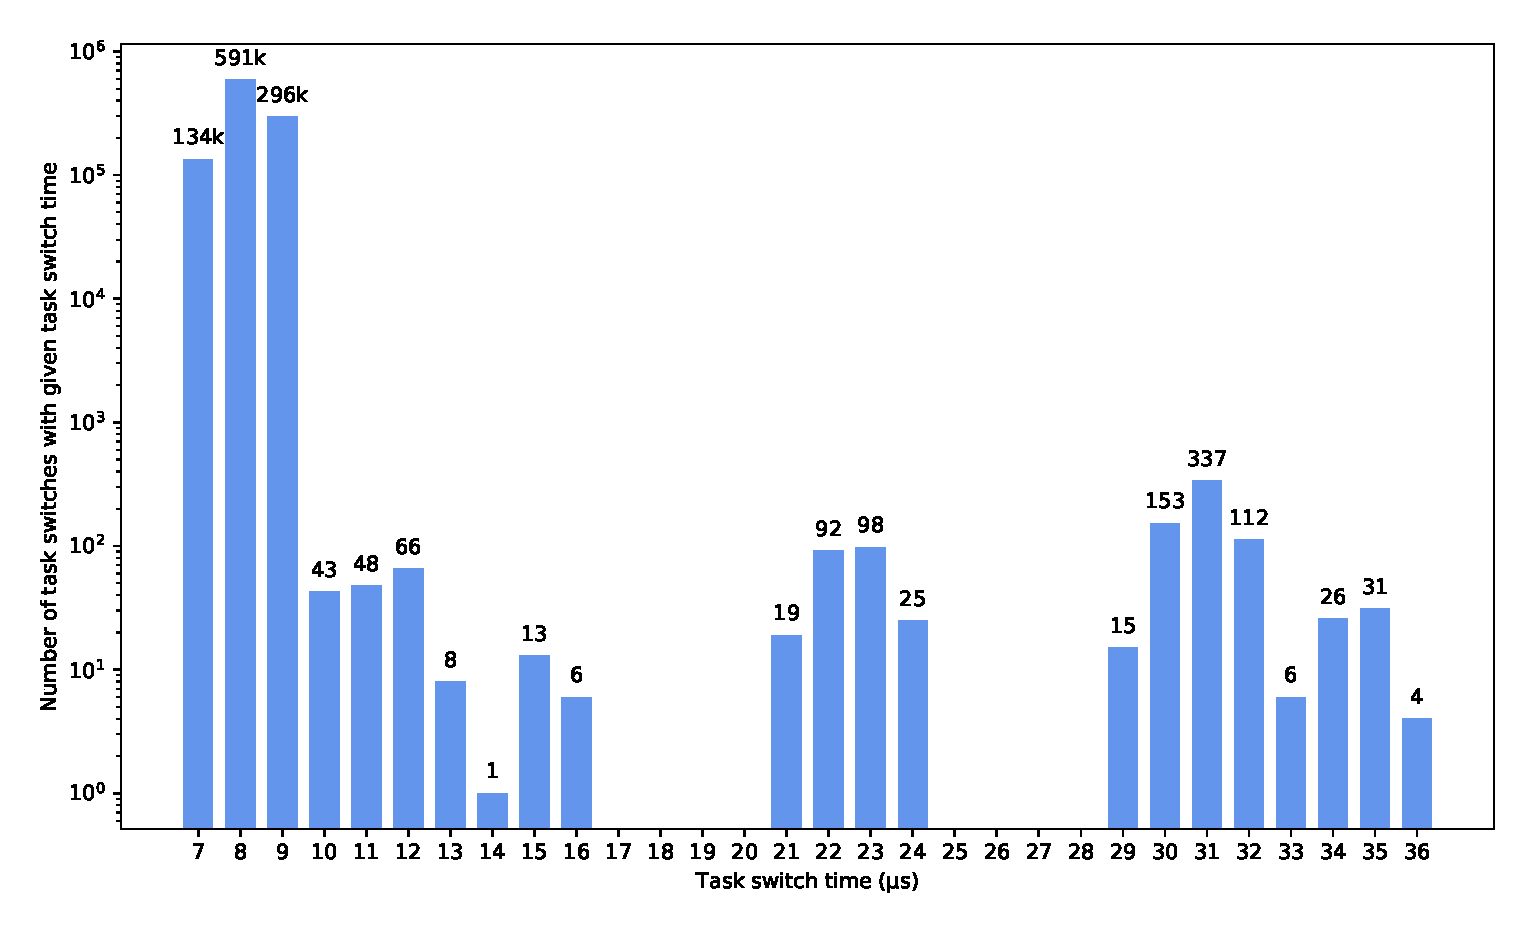
\includegraphics[width=\textwidth]{figures/task_switch_time.eps}
    \caption{A histogram of task switch time between round-robin tasks (mean 8.17µs; std. dev. 0.90µs). Total samples: 1,024,000.}
    \label{fig:rrhist}
\end{figure}

\subsection{\ucosiii scheduler: task switch time as the number of priorities increases}
As the number of priorities increases, the size of the priority bitmap increases linearly. Since we search the priority bitmap each time we perform a task switch, we would expect task switch time to increase linearly as well. In figure~\ref{fig:prioboxplot}, a set of box plots of task switch time is shown, for a varying number of priorities. For each number of priorities, 32 tasks were spaced evenly in the priority space, and the time to switch between them was measured for each task switch for a duration of five seconds. As expected, the mean task switch time increases linearly (visible as a curved line in this log-log plot due to the non-zero y-intercept). Additionally, the variance increases greatly as the number of priorities increases.

\begin{figure}[htpb]
    \centering
    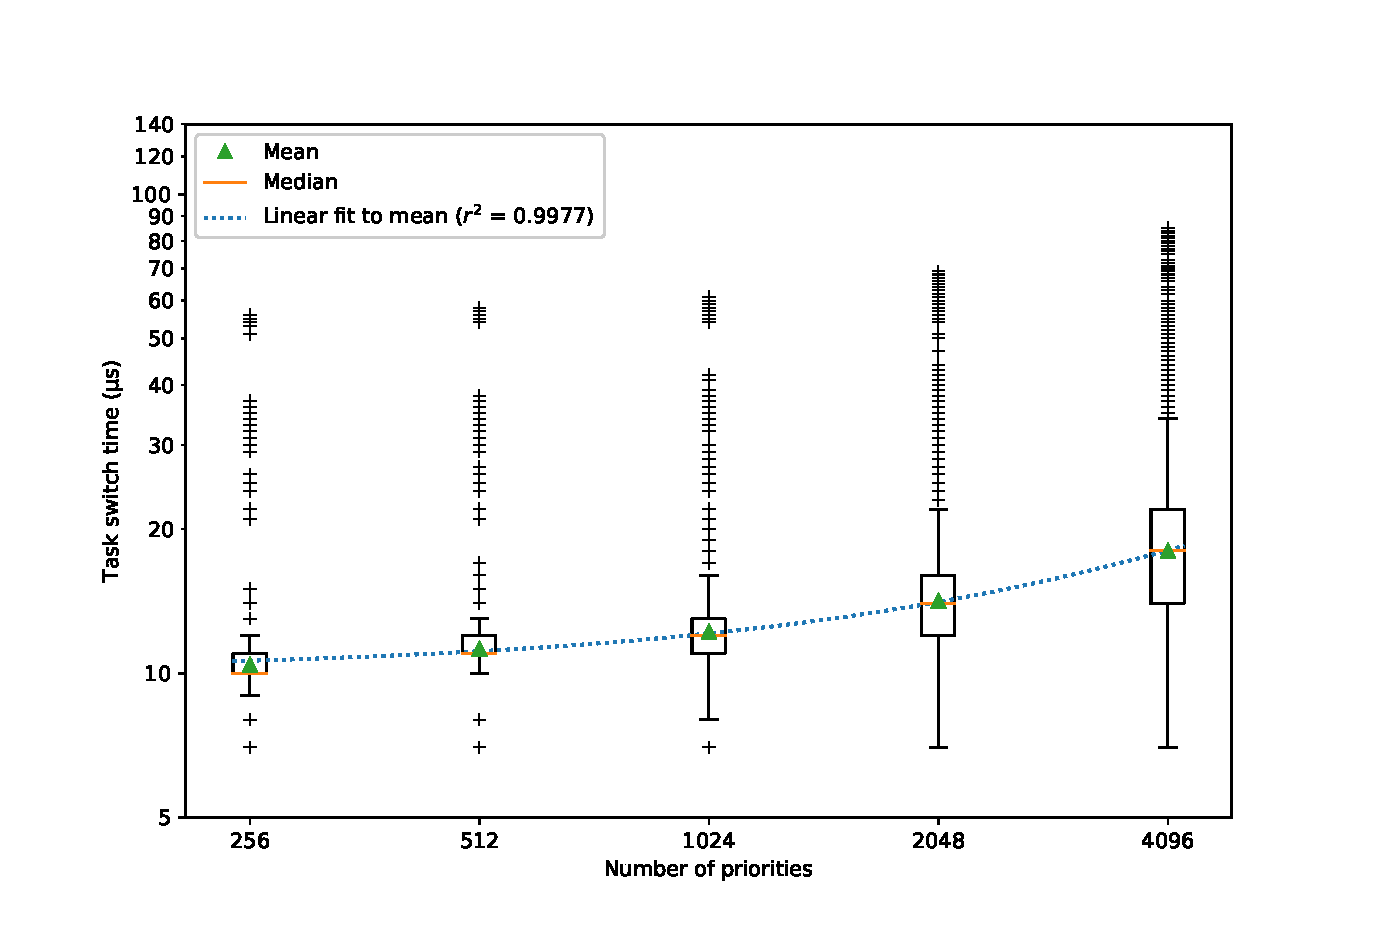
\includegraphics[width=\textwidth]{figures/boxplot.eps}
    \caption{\ucosiii scheduler: box plots of task switch time as the number of priorities increases. As task switches were measured over a fixed period of time, the number of samples for each box plot varies, from a minimum of 547,535 to a maximum of 938,926.}
    \label{fig:prioboxplot}
\end{figure}

\subsection{EDF scheduler: task switch time as number of tasks increases}
The task switch time of the EDF scheduler is evaluated as the number of tasks increases, as the number of tasks influences the time taken to maintain the heap property. We expect the time to increase logarithmically as the number of tasks increases, since heap insertion and deletion occurs in $\log n$ time. Results can be seen in figure~\ref{fig:edfboxplot}. We can see that task switch time is in roughly the same order of magnitude as the priority-based \ucosiii scheduler, with average task switch times in the tens of milliseconds.

The code used to run the task sets in this experiment can be found in the \code{edf-task-switch-time} branch -- a separate branch was created as EDF functions were instrumented, and the test code could not be cleanly moved into a separate app.

\begin{figure}[htpb]
    \centering
    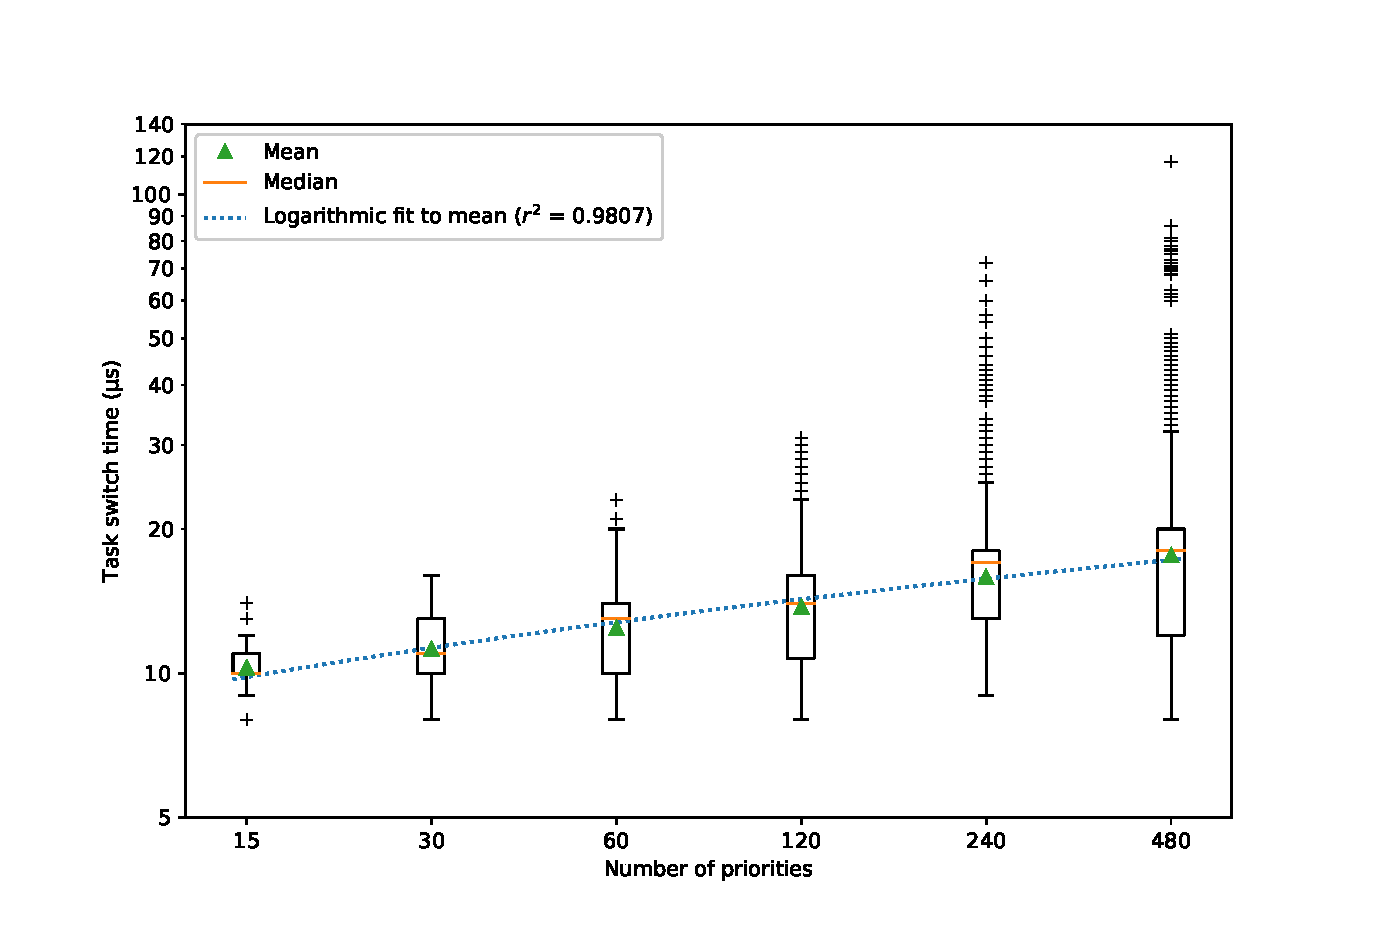
\includegraphics[width=\textwidth]{figures/edfboxplot.eps}
    \caption{EDF scheduler: box plots of task switch time as the number of tasks increases. Each box plot contains 10,000 samples.}
    \label{fig:edfboxplot}
\end{figure}

\section{Task set schedulability}
In this experiment, the new EDF scheduler is compared to the built-in scheduler when it comes to task set schedulability. Random task sets were generated and EDF schedulability was analyzed using the processor demand criterion, then confirmed by running the task sets on hardware. The same task sets were run using the Rate Monotonic algorithm and the built-in fixed priority scheduler. The method by which task sets were generated and run is discussed below.

\subsection{Determining worst-case execution times}
As discussed in the chapter on scheduling, when using guarantee-backed scheduling, an accurate worst-case execution time estimation for tasks is paramount to ensure that the provided guarantees actually have meaning. The same is true when evaluating scheduling performance. However, worst-case execution time estimation is a difficult task for even simple code, and in these experiments, I would like to greatly vary task sets, requiring me to perform worst-case execution time analysis for many task sets. Therefore, I have chosen to simulate actual tasks by executing instructions which do not perform any useful work, but have very predictable timing characteristics. These timing characteristics can be found in chapter 16 of the ARM Technical Reference Manual for the Pi's ARM1176JZF-S processor\cite{arm:arm1176}.\\


\begin{lstlisting}
wait_for_cycles:
    lsr r0,r0,#1
loop$:
    subs r0, r0, #1
    bne loop$
    bx lr
\end{lstlisting}

\begin{enumerate}
    \item The \code{wait_for_cycles} subroutine waits for approximately $r_0$ cycles. A description of the cycle count of the used instructions is as follows;
    \item The \code{lsr} instruction is syntactic sugar for a \code{mov} instruction with included shift, and therefore takes a single cycle\cite[p. 16-7]{arm:arm1176}. It requires its source register as an early register, but that should be no issue as this is the first instruction in the function.
    \setcounter{enumi}{3}
    \item Data processing instructions not targeting the program counter and without included shifts, such as this \code{subs} instruction, take a single cycle\cite[p. 16-7]{arm:arm1176}.
    \item Branch instructions such as \code{bne} have complex timing characteristics, since the ARM1176JZF-S processor includes both a static and a dynamic branch predictor, as well as a return prediction stack\cite[p. 16-2]{arm:arm1176}. Let us assume a scenario where we want to wait for a number of cycles that is greater than one.

    The first time this branch executes and when it is not in the 128-entry dynamic branch predictor cache, it will take 4 cycles, as it will be correctly predicted to be taken by the static branch predictor, which predicts that backward branches are always taken\cite[p. 5-5]{arm:arm1176}.

    After this, it will be set to be weakly taken in the dynamic branch predictor. This correct prediction allows the branch to take a single cycle\footnote{If folded out, the branch could take zero cycles. Since branch folding is hard to predict, however, my startup code disables branch folding.}\cite{arm:arm1176}.

    After the last iteration, the branch will be mispredicted, and as the subtraction instruction directly precedes the branch instruction, this incurs a cost of 6 cycles.
    \item The return instruction takes 4 or 5 cycles depending on whether the code is interrupted - if it is, the return stack will most likely be empty and therefore cause an extra cycle.
\end{enumerate}

The cycle count for the given instructions could vary based on presence in the instruction cache or other architectural buffers (such as the instruction prefetch buffer). Most important, however, is the timing of the instructions in the inner loop, as they account for the bulk of the cycles used. Experimentally, the 2-cycle inner loop behavior is verified in \code{apps/waittest/app.c}.

One issue with using cycles to wait for a given period of time is the variability of the Pi's clock speed. The Pi will, however, only throttle the clock speed in two cases; when an undervoltage is detected (this occurs when the power supply cannot supply 5 volts at the required amperage, so the voltage drops) or when the core temperature gets above 80 degrees\cite{rpi:gpuclockpower}. Measuring the GPIO voltage during system stress reveals that my power supply can consistently supply five volts. The second case does not occur on first-generation Pis due to its low-power processor (later generations have higher clock speeds and are multi-core chips, and therefore have a larger thermal output and are at higher risk of overheating). Therefore, we can rely on the system clock staying constant.

\subsection{Generating task sets}
To measure task set schedulability, a range of random task sets was generated. The parameters for these task sets were as follows:

\begin{itemize}
    \item \textbf{Target processor utilization} varied between 65\% and 100\%, skewing slightly toward higher processor utilization since fewer randomly generated task sets hit the higher processor utilization. In the end, the accepted task set with the highest processor utilization had $U \approx 0.985$.
    \item The \textbf{task utilization} was picked uniformly between zero and the remaining available processor utilization
    \item The \textbf{period} was chosen between 250 and 1000 milliseconds, in multiples of 10 to get a tractable hyperperiod.
    \item The \textbf{worst-case execution time} of a task was derived by multiplying a task's utilization with its period.
    \item The \textbf{relative deadline} of a task was generated by subtracting a third of the difference between the period and the worst-case execution time.
    \item The \textbf{number of tasks} varied between 5 and 11, with a mean of 5.78 tasks in a task set.
\end{itemize}

\noindent Additionally, the \ucos tick task was added to the task sets when computing the scheduling guarantee. As noted in the chapter on implementation, parameters of the tick task were estimated as $T_{\text{tick}} = 1$ tick, $C_\text{tick} = 50$\textmu s , $D_\text{tick} = 250$\textmu s.

After task generation, task sets that had fewer than 5 tasks or a hyperperiod that was longer than 100 seconds were excluded. This left \totalsets{} task sets, which were partitioned into \totalsuccess{} task sets that passed the schedulability guarantee and \totalfailure{} task sets that did not. These task sets were subsequently run.

The way the generated task sets were distributed across the processor utilization spectrum can be seen in figure~\ref{fig:tasksetsdist}.

\begin{figure}[htpb]
    \centering
    \hspace*{-1.6cm}
    \begin{minipage}{0.62\textwidth}
        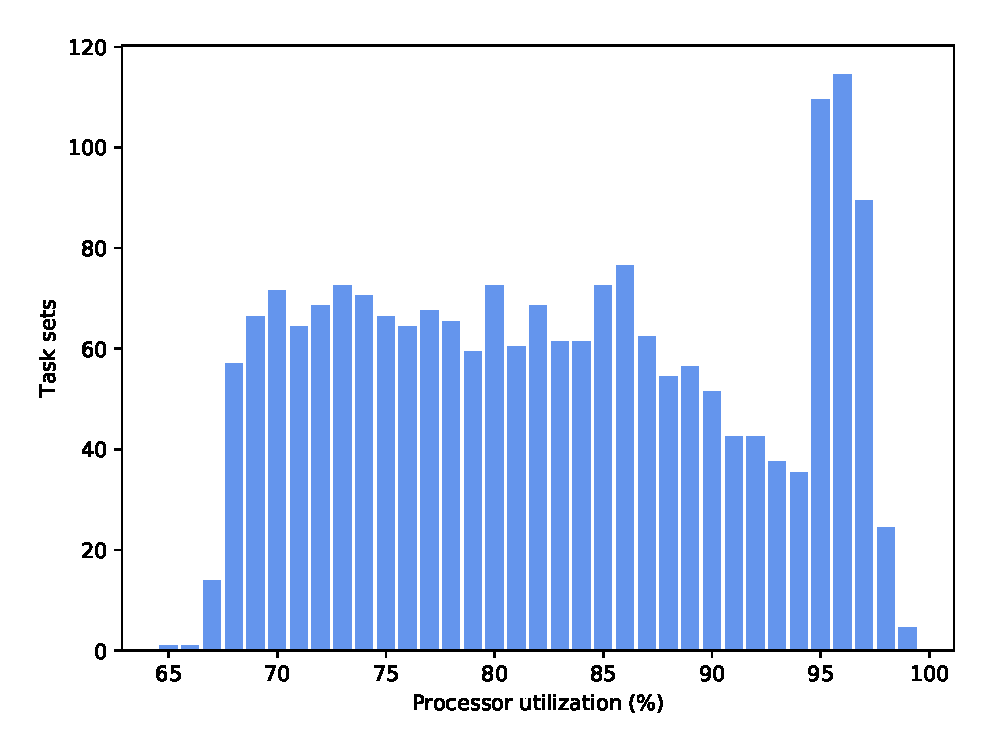
\includegraphics[width=\textwidth]{figures/guarantee_passed_distribution.eps}
    \end{minipage}%
    \begin{minipage}{0.62\textwidth}
        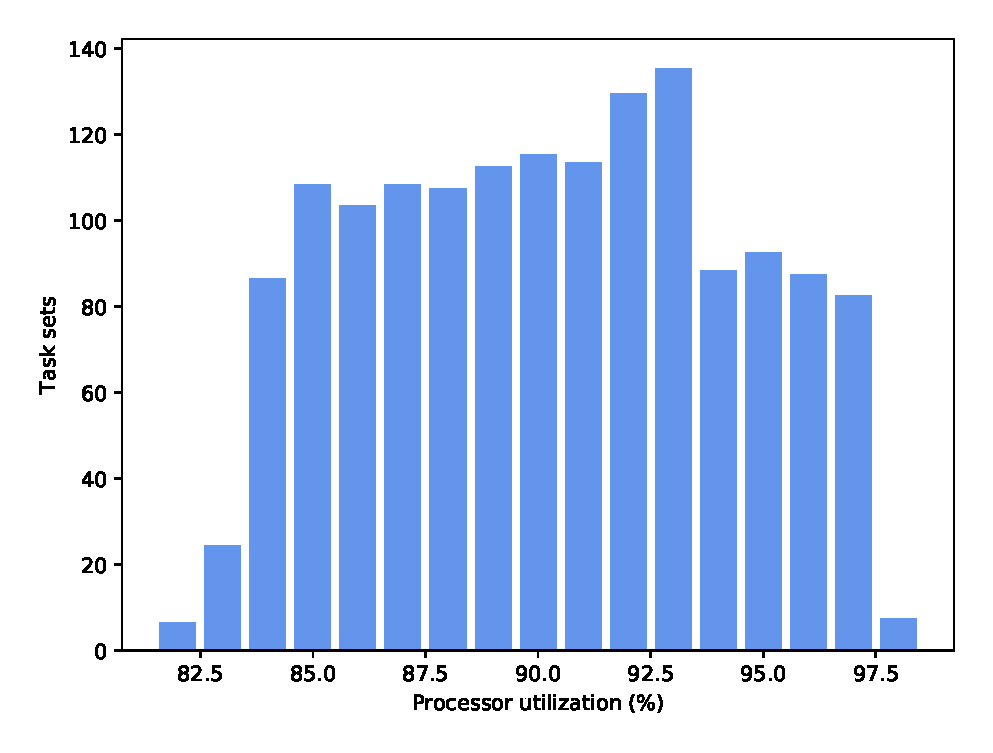
\includegraphics[width=\textwidth]{figures/guarantee_failed_distribution.eps}
    \end{minipage}
    \caption{The distribution of the task sets which passed (left) and failed (right) the EDF schedulability guarantee, as rounded to the nearest whole percentage.}
    \label{fig:tasksetsdist}
\end{figure}

\subsection{Running task sets}
To validate the schedulability guarantee, the task sets were executed on the real hardware. To evaluate the practical schedulability of a task set, the task set was run until the end of its hyperperiod, or until its first deadline miss, whichever came first. Since, in all of these task sets, the relative deadlines of tasks are smaller or equal to their period, when the hyperperiod passes, the schedule repeats itself, and the task set does not need to be run any longer to evaluate schedulability.

The data collection was done automatically, by restarting the Raspberry Pi using its hardware watchdog after task set execution, compiling a new kernel with the next task set, and loading that over the serial connection. Execution was then monitored, marking a task set as `failed' when a deadline miss was reported, and as `successful' otherwise.

\subsubsection{Results for the Rate Monotonic scheduler}
Of the \totalsuccess{} task sets that passed the EDF schedulability guarantee, 1103 task sets missed a deadline when scheduled under the Rate Monotonic algorithm, and 922 task sets ran without any deadline misses. Of the rejected task sets, \rmfailurepassed{} task sets ran without any deadline misses, whereas \rmfailurefailed{} task sets missed a deadline. The success and failure rate can be seen in figure~\ref{fig:rmresults}. We can see a crossover point at $U \approx 80\%$, where the amount of task sets that fail to execute without missing a deadline exceeds the amount of task sets that run successfully.

\begin{figure}[htpb]
    \centering
    \hspace*{-2.4cm}
    \begin{minipage}{0.62\textwidth}
        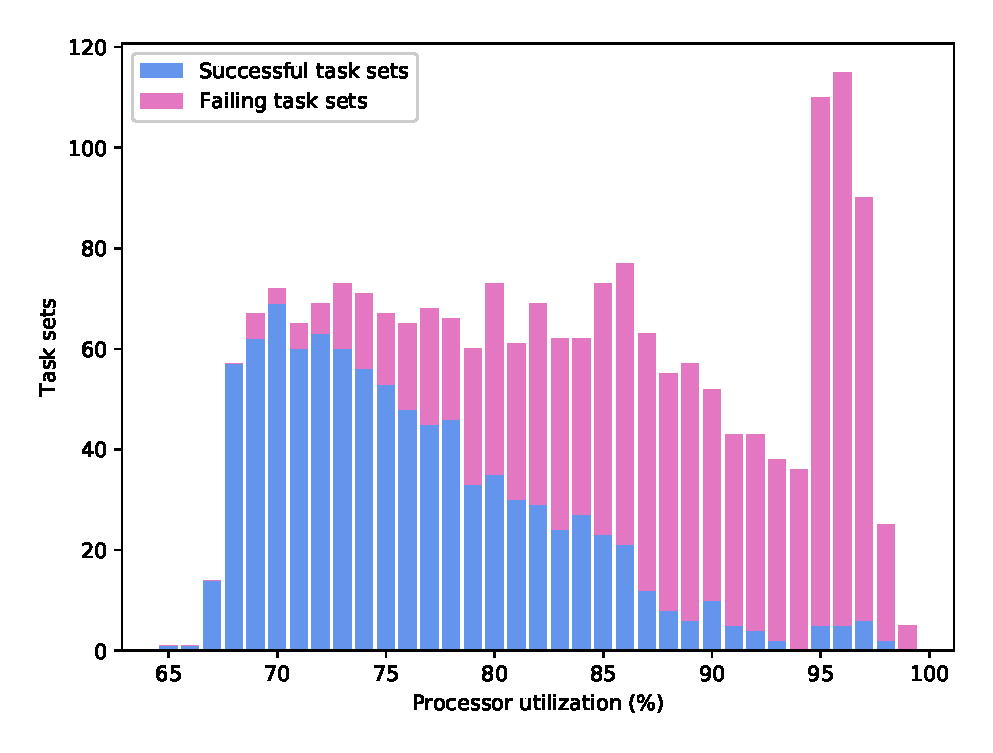
\includegraphics[width=\textwidth]{figures/rm_guarantee_pass_percentage.eps}
    \end{minipage}%
    \begin{minipage}{0.62\textwidth}
        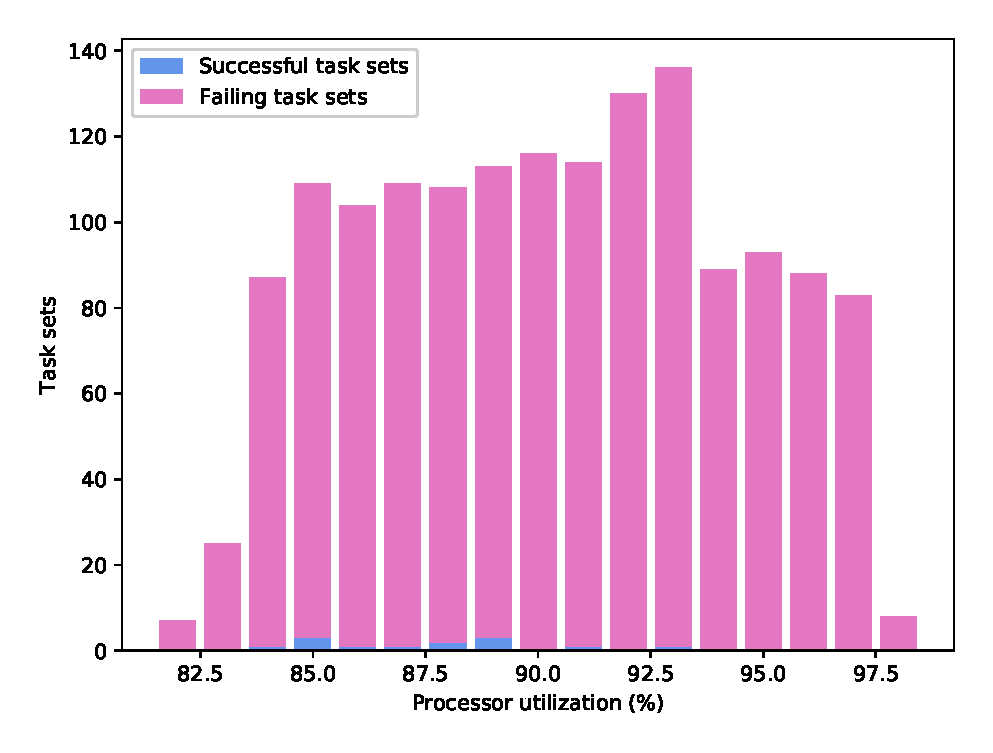
\includegraphics[width=\textwidth]{figures/rm_guarantee_fail_percentage.eps}
    \end{minipage}
    \hspace*{-2.4cm}
    \begin{minipage}{0.62\textwidth}
        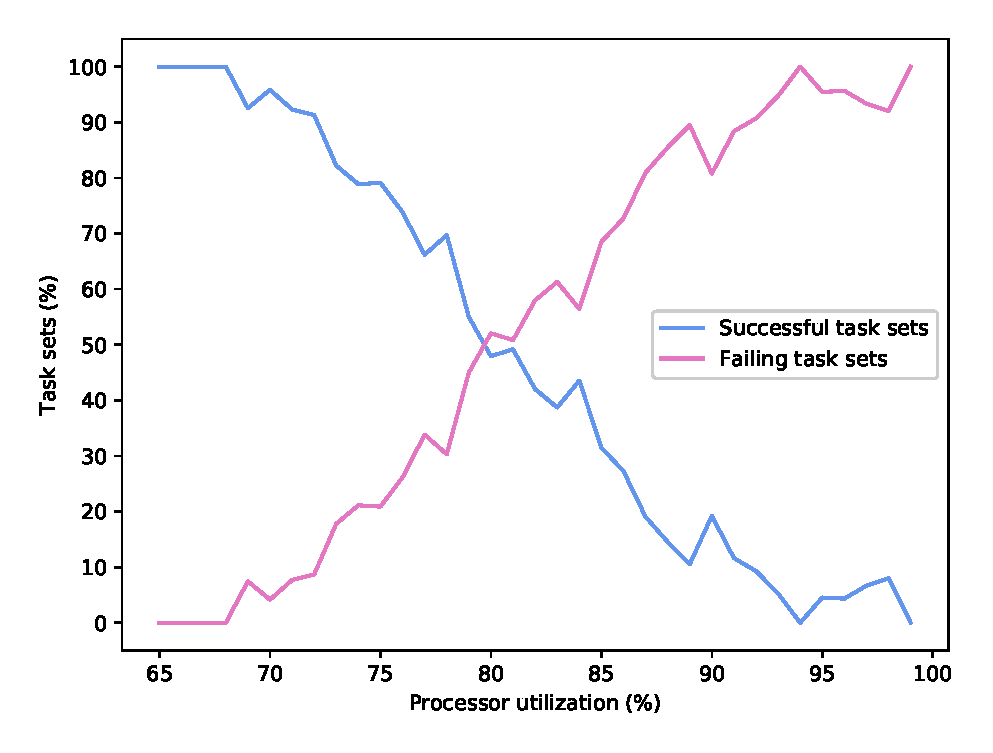
\includegraphics[width=\textwidth]{figures/crossover_rm_succ.eps}
    \end{minipage}%
    \begin{minipage}{0.62\textwidth}
        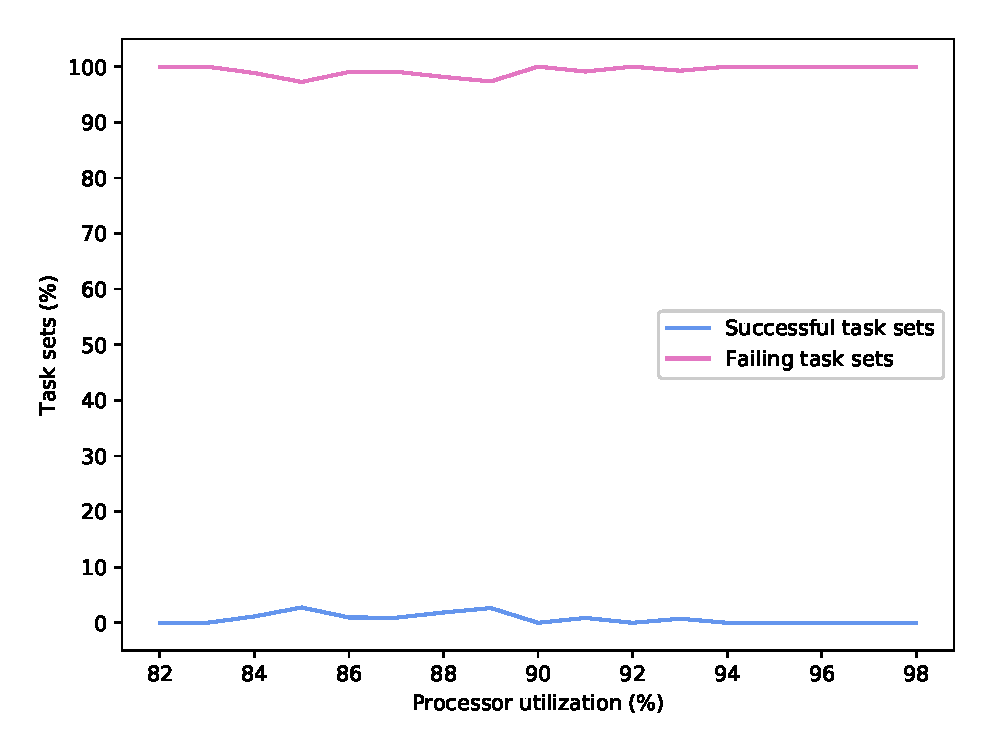
\includegraphics[width=\textwidth]{figures/crossover_rm_fail.eps}
    \end{minipage}
    \caption{Results for the RM scheduler. Top left: success/failure stack plot for tasks that passed the EDF schedulability guarantee. Top right: success/failure stack plot for tasks that failed the EDF schedulability guarantee. Bottom left and bottom right: success/failure percentage for tasks that passed and failed the EDF schedulability guarantee, respectively. Task set processor utilization is rounded to the nearest percentage.}
    \label{fig:rmresults}
\end{figure}

\newpage
\subsubsection{Results for the Earliest Deadline First scheduler}
All \totalsuccess{} task sets that passed the schedulability guarantee were run without any deadline misses. Of the \totalfailure{} rejected task sets, \edffailurepassed{} ran without any deadline misses, whereas the other \edffailurefailed{} missed at least one deadline. The results for the EDF scheduler can be seen in figure~\ref{fig:edfresults}. Of note is the fairly consistent 20\% success rate among tasks that failed the scheduling guarantee. This indicates an overestimation of task parameters, most likely those of the \ucos Tick Task.

\begin{figure}[htpb]
    \centering
    \hspace*{-1.6cm}
    \begin{minipage}{0.62\textwidth}
        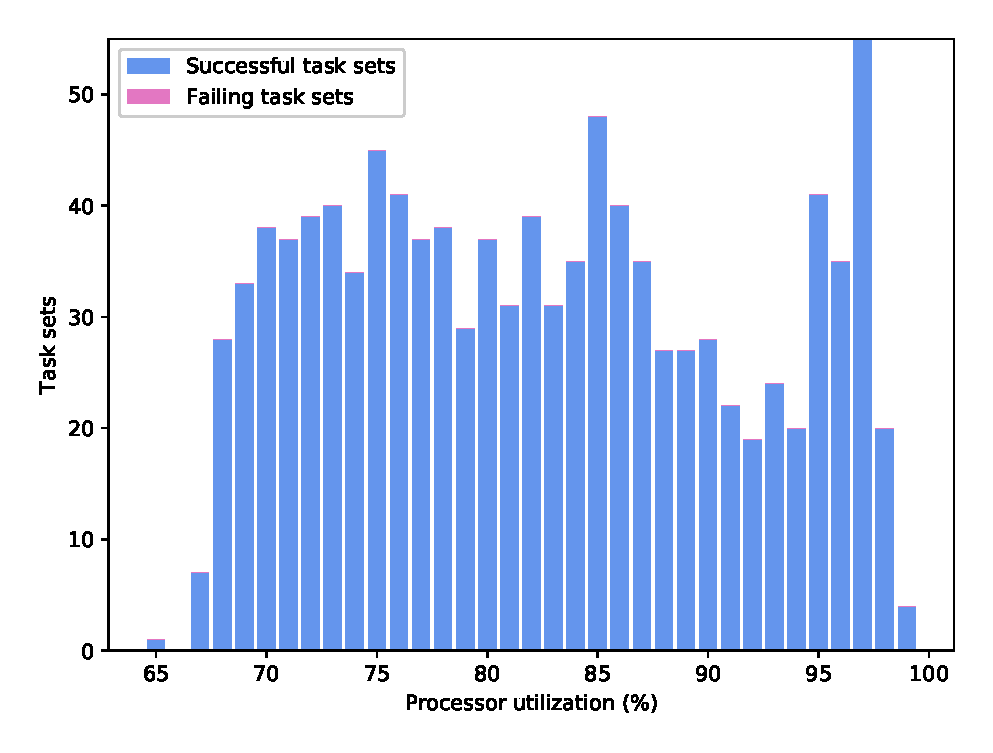
\includegraphics[width=\textwidth]{figures/edf_guarantee_pass_percentage.eps}
    \end{minipage}%
    \begin{minipage}{0.62\textwidth}
        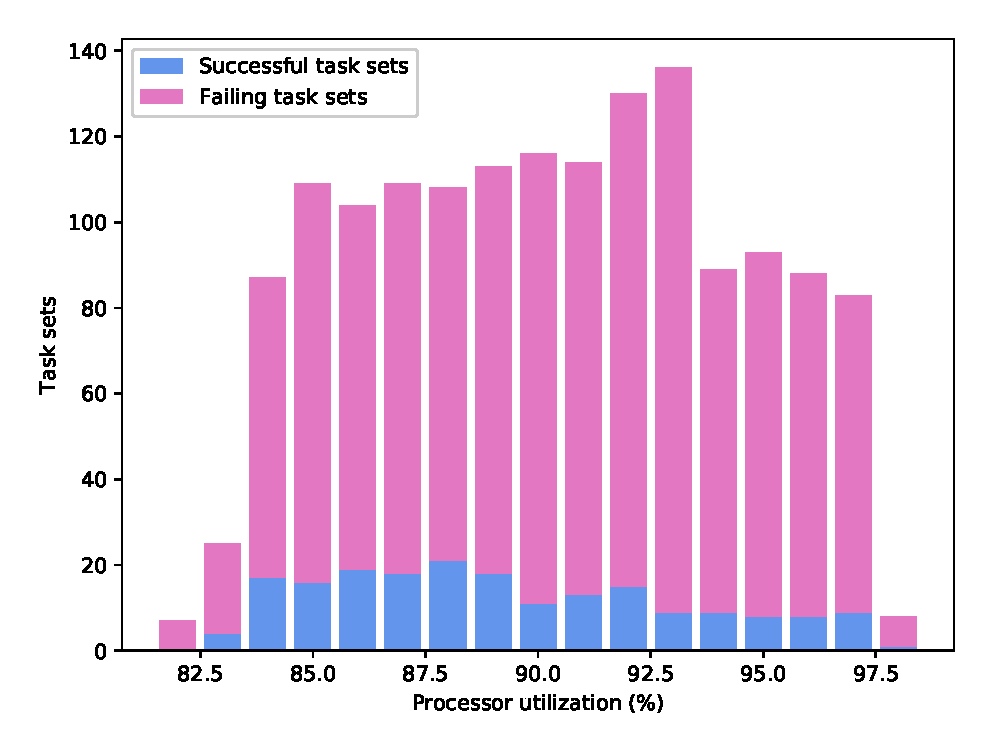
\includegraphics[width=\textwidth]{figures/edf_guarantee_fail_percentage.eps}
    \end{minipage}
    \hspace*{-1.6cm}
    \begin{minipage}{0.62\textwidth}
        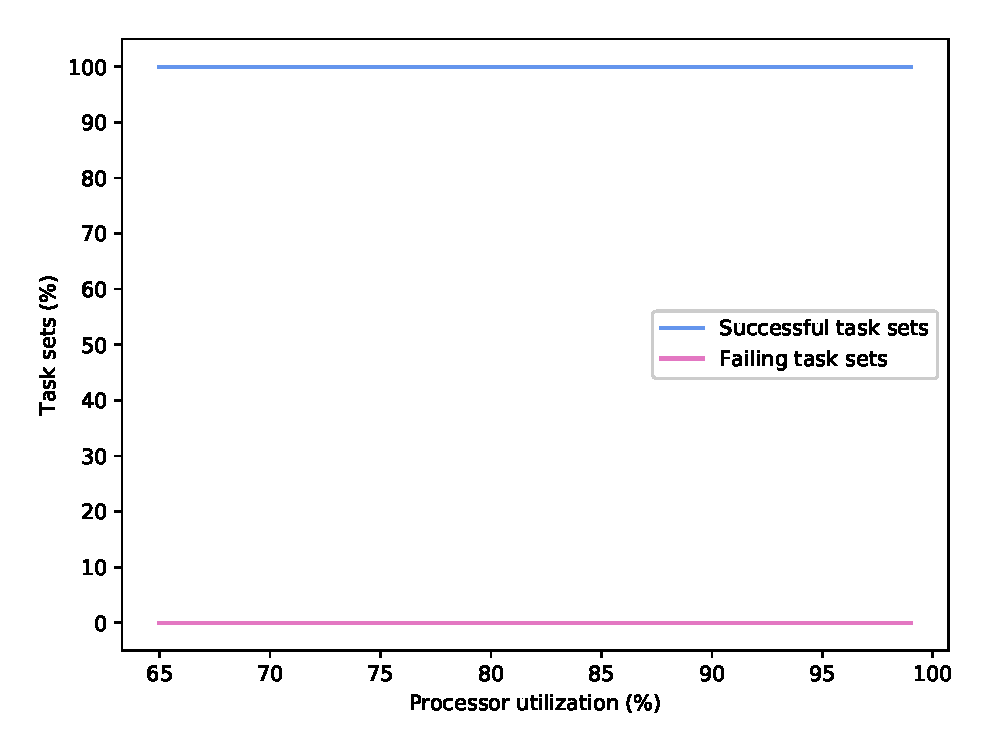
\includegraphics[width=\textwidth]{figures/crossover_edf_succ.eps}
    \end{minipage}%
    \begin{minipage}{0.62\textwidth}
        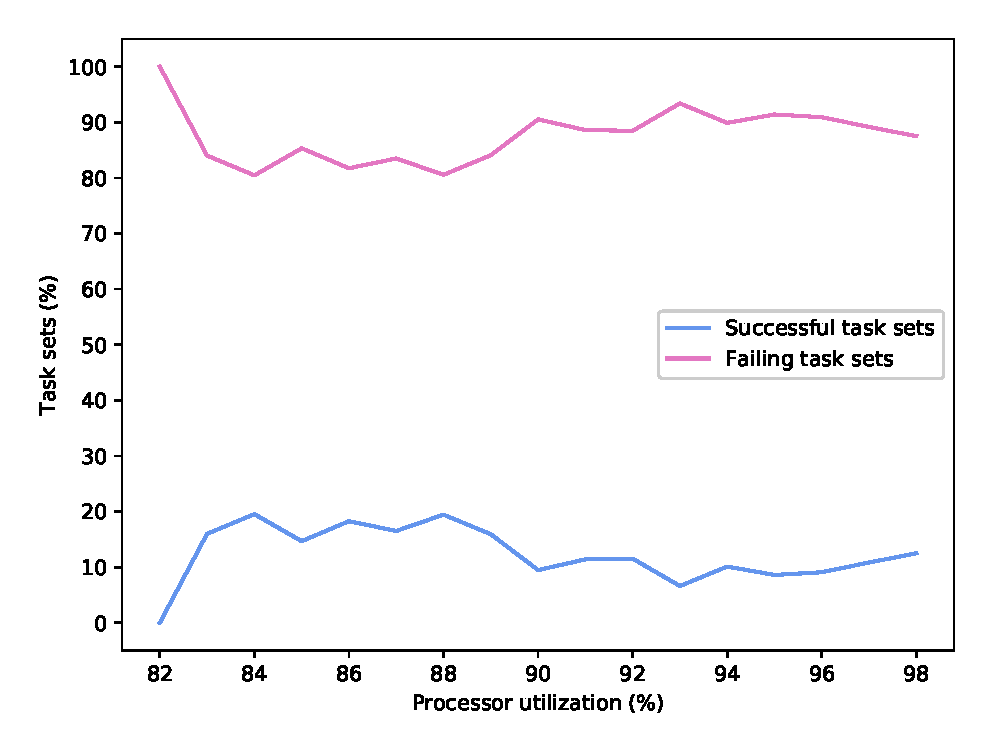
\includegraphics[width=\textwidth]{figures/crossover_edf_fail.eps}
    \end{minipage}
    \caption{Results for the EDF scheduler. Top left: success/failure stack plot for tasks that passed the EDF schedulability guarantee. Top right: success/failure stack plot for tasks that failed the EDF schedulability guarantee. Bottom left and bottom right: success/failure percentage for tasks that passed and failed the EDF schedulability guarantee, respectively. Task set processor utilization is rounded to the nearest percentage.}
    \label{fig:edfresults}
\end{figure}

